\label{chapter:hla1}

In this chapter, we discuss our approach compared to existing studies for labeling abstraction nodes. In Section \ref{hla1:intro} and \ref{hla1:motivation}, we introduce important concepts, related works and what we did to advance them. Section \ref{approach} presents our approaches for cluster naming, Section \ref{Experimental} describes our experimental design, 
Section \ref{results} presents the technique evaluations,
and finally, Section \ref{conclusion} summarizes the chapter by mentioning our future direction.  


\section{Introduction}
\label{hla1:intro}
Understanding the source code of a software system is a prevalent and vital task for the developers because many software engineering tasks depend on program comprehension \cite{cornelissen2009systematic, gilmore1991models, xie2016revisit, feng2018hierarchicalExecutionComprehension}. It is difficult for an individual developer to develop an enterprise software system on their own. Therefore, when someone is assigned to a task or join a development team, they need to understand the existing system to get used to the system. This program comprehension involves a lot of browsing back-and-forth between different granularity levels of the codebase. To reduce developers' effort to comprehend program artifacts, a lot of research is going on in the field of program comprehension \cite{feng2018hierarchicalExecutionComprehension, gharibi2018automaticStaticCluster, kulkarni2014supporting, izu2019program}. An abstract representation of the target software system can easily guide the exploration of low-level source code depending on developers' maintenance tasks. One of the approaches is to generate dynamic logs of function executions while running an existing system on different test cases. The logs can then be used with other methods to produce a suitable output for developers to comprehend the software system \cite{feng2018hierarchicalExecutionComprehension}.
Moreover, most of the dynamic approaches generate dynamic call graphs from the generated dynamic logs of various system scenarios. However, the problem with dynamic call logs is that they only consider the function executions invoked during the dynamic log generation of a target system based on the test cases. As a result, not all the functionalities of the target system are considered during the codebase investigation. Another problem with dynamic logs is that they generate billions of data points, which are mostly redundant. If someone wants to abstract the whole system for comprehension purposes, then using dynamic logs does not help much to cover the entire system.
On the other hand, a static call-graph can be generated by extracting caller-callee relationships from source files. The benefit of a static call graph is that it is possible to have a target system's overall functionalities. The static call graph also resolves the problem of redundant data of the log generations.



A large portion of a developers' development time is devoted to understanding existing source codes \cite{corbi1989program, minelli2015know, ko2006exploratory}. Because without knowing the cognitive relation between source code with higher-level system functionalities, it is difficult to perform different software maintenance tasks (e.g., debugging, feature addition, refactoring, and testing). So, browsing back-and-forth between different source files of a system is widespread among developers to comprehend an existing system. What developers usually do is that they first look for the name of a source file's functions to understand the intention of the functions \cite{de2012IRMethodsArtifacts, starke2009searching}. Therefore, the function names can be utilized for abstracting a system's higher-level functionalities. Moreover, existing studies suggested that \cite{salah2005scenariographerReverseEngineering,pradel2009automaticUseageSpecification} sequence of function invocations can help extract usage scenarios or higher-level functionalities of a target system. Hence, having a tool that visualizes the cognitive mapping between source code and high-level functionalities and allows browsing through source code in a more informed way would help developers.

% \subsection{Why is it hard? (E.g., why do naive approaches fail?)}
% complex source code base, difference between natural language and source code, different characteristics of different language and frameworks, huge amount of data to summarize, creating priority
Manually browsing source code for locating concepts is a laborious task. As a consequence, a lot of existing studies have been done to map concepts with source code using dynamic execution logs. However, very few studies considered static call graphs and emphasized function names. Gharib \textit{et al.} \cite{gharibi2018automaticStaticCluster} proposed a technique based on static call graphs where concepts are mapped with source codes. The authors have presented a whole subject system as a tree where nodes represent concepts of the system. However, they have only applied the TFIDF technique to extract the concepts of a particular codebase. During concept location, they have just considered the name of the function as term. Another drawback of their study is that they have not conducted any use case analysis from users' perspectives. So how developers will be comprehending the source code of a software system is absent in the study for real-world cases.

These limitations of the existing work motivated us to investigate more details on the potential of this approach. We have applied one information retrieval technique, TFIDF, and two topic modeling techniques (LDA and LSI). In the previous study \cite{gharibi2018automaticStaticCluster}, the full function name is treated as a term for the TFIDF technique. Here, we introduce words in function names as another variation. In total, we have six techniques to evaluate, as each technique mentioned above has two variations (function name and words in function name) result. We have also performed a small scale user-study with five developers. We have used 12 clusters from three subject systems as use cases to evaluate our approaches. Developers have rated the summaries generated by each technique and provided their summary of each use case, which we used to assess our automatic techniques using the Pyramid metric. From our investigation, we have found that automatic labeling using TFIDF for words in method names as term variation has an average of 64\% overlap with manual labeling of participants. LDA and LSI received 37\%, and 23\% overlap accordingly. We have also found that words in function name variants got a minimum of 5\% more preference rating compared to function name variants from developers. 

In summary, our contributions are:
\begin{itemize}
  \item We adopted two topic modeling techniques to name nodes of the abstract code summary tree. 
  \item We introduce using words in the function name as a term for information retrieval techniques.
  \item We have conducted small scale user study to evaluate the proposed techniques.
\end{itemize}



\section{Motivational Example}
\label{hla1:motivation}

This section is presented with a motivational example of real-world scenarios. Suppose Bob joined a new company X as a Junior Software Developer. He needs to work on a software project which is being developed for more than six years. He must have a cognitive mapping between source code artifacts and high-level concepts of the software project, which will boost his integration to the project. To get an understanding of the project, he can use the Call graph of the project, which visualizes functional dependency.

\begin{figure*}[h]
  \centering
  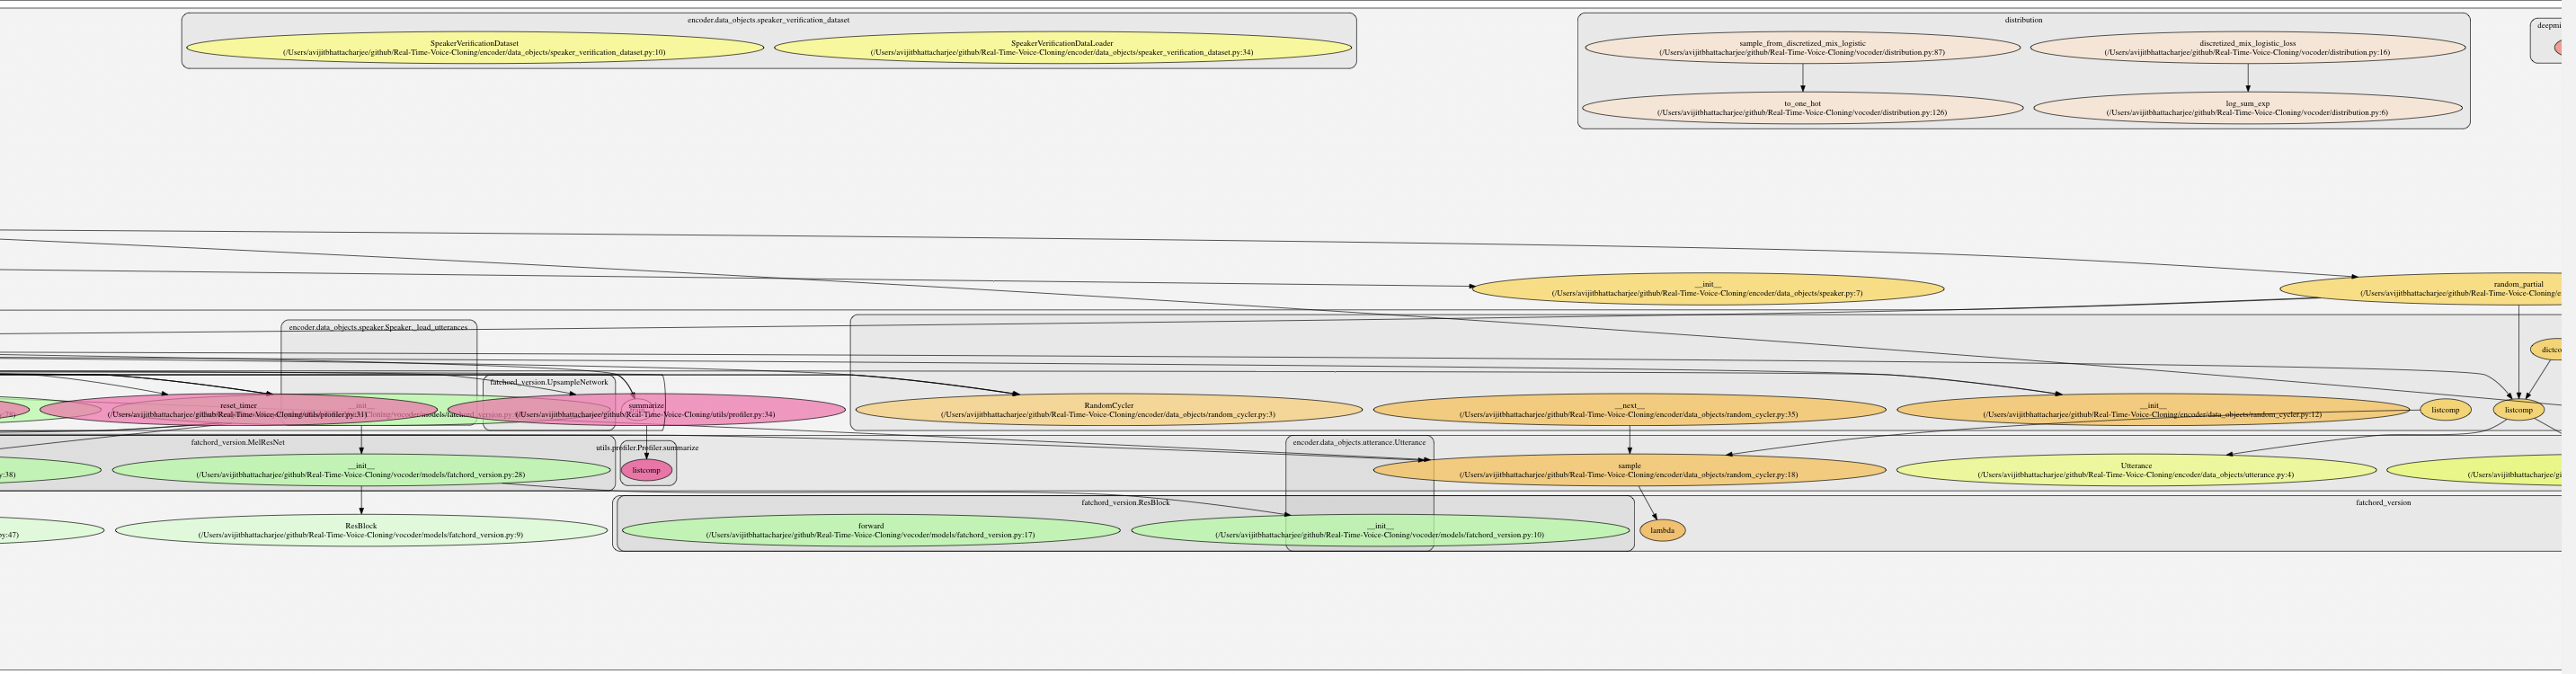
\includegraphics[width=\columnwidth]{figures/hla1/realTime.png}
  \caption{A portion of the Call graph of Real-Time-Voice-Cloning project by Pyan}~\label{fig:realTime}
\end{figure*}

However, in Figure \ref{fig:realTime} we can see a portion of the large call graph generated using Pyan \cite{pyan} for Real-Time-Voice-Cloning \cite{realTime} project. This presentation is very complex and hard to comprehend. Furthermore, if Bob has any particular Software Engineering task to do, first, he needs to locate the concept in source code. Locating source code artifacts relevant to the specific task will help Bob do his task faster. Therefore, our approach starts from this complex call graph and extracts concepts from execution paths in various hierarchical levels. Using the proposed approach, Bob can explore concepts from top-to-bottom, which at the end map to execution paths and the name of functions for smooth inquiries. 


 
 
% \vspace{6mm}
\section{Approach}

\begin{figure*}[tb]
  \centering
  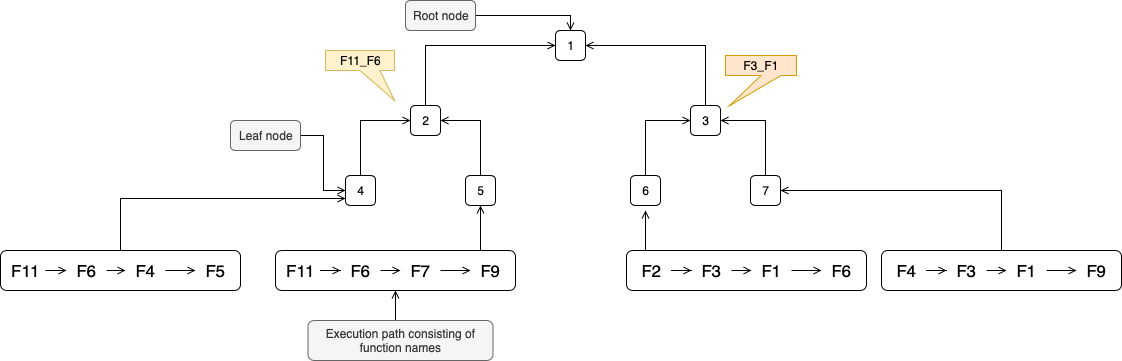
\includegraphics[width=\columnwidth]{figures/hla1/visual_tool_static_call_graph-2.png}
  \caption{Structure of an abstract code summary tree}~\label{fig:hla1_motivation}
\end{figure*}
In this section, we discuss two significant steps in our approach with a brief discussion. First, in Section \ref{hla1:approach_acs}., we described six steps to get the cluster tree of a subject system. Second, in Section \ref{hla1:node_title}, we explain how we used different information retrieval techniques to label nodes of the abstract code summary tree. Data collection for evaluating the approach is depicted in algorithm \ref{hla1:alg:overall}.

\label{approach}

\begin{algorithm}
    \SetKwInOut{Input}{Input}
    \SetKwInOut{Output}{Output}
    
    \underline{Call Graph to abstract code summary tree} $(call graph)$\;
    
    \Input{Call graph}
    \Output{Abstract code summary tree}
    \For{Iterate each node in the call graph}
    {
        \If{ $Number\_of\_Incoming\_Degree(node) == 0$}
        {
            entryNodes.append(node);
        }
        \If{$Number\_of\_Outgoing\_Degree(node) == 0$}{
            exitNodes.append(node);
        }
    } 
    \For{$i\gets1$ \KwTo $entryNodes.length$ \KwBy $1$}
    {
        \For{$j\gets1$ \KwTo $exitNodes.length$ \KwBy $1$}
        {
            execution\_paths.append($simple\_DFS\_path(i, j)$);
        }
    }
    \For{$i\gets1$ \KwTo $execution\_paths.length$ \KwBy $1$}
    {
        \For{$j\gets1$ \KwTo $execution\_paths.length$ \KwBy $1$}
        {
            $distance\_matrix[i][j]$ = $consine\_similarity(i,j)$;
        }
    }
    $cluster\_tree$ = $create\_cluster\_tree(distance\_matrix)$;
    
    $abstract\_code\_summary\_tree$ = $generate\_label\_for\_each\_node(cluster\_tree)$;
    
    return $abstract\_code\_summary\_tree$;
    \caption{Constructing Python source code to an abstract code summary tree}
    \label{hla1:alg:overall}
\end{algorithm}

% \vspace{4mm}
\subsection{Abstract Code Summary (ACS) Tree}
\label{hla1:approach_acs}
The call graph is a visual representation of the relationships between the functions of a project. We adopt static call graphs, which are generated by analyzing source code. As the static call
graphs capture all function calls of a target system, we
choose to abstract the target system. Previous studies suggested that function names contain significant abstraction of source code. Thus, we emphasize mining concepts by analyzing function names in the static call graph.
As we want to capture and abstract the overall system's high-level concepts, therefore, the decision for adopting a static call graph as a building-block of our approach and using function names for concept location is well-justified.  

In Figure \ref{fig:hla1_motivation}, we present the structure of our proposed abstract code summary tree. The leaf nodes of this tree are directly mapped to the execution paths. The execution paths are a list of function names executed sequentially during the execution of a software system. For instance, node 5 is mapped to the execution path where \texttt{ F11, F6, F7, and F9} are called sequentially. Similarly,  in this scenario, all the four-leaf nodes 4, 5, 6, and 7 are mapped to four execution paths or function call sequences. Node 1, 2, and 3 are intermediate nodes of the tree. Naming these intermediate nodes analyzing the execution paths that resides under them might reduce the need to go through in detail about their functionalities. In the figure, node 2 has been named \texttt{F11\_F6}, and node 3 has been named as \texttt{F3\_F1}  by analyzing the function names in the execution paths under those nodes. If we find a proper naming technique that can map concepts in source code with different granularity levels, this approach can make developers program comprehension tasks more flexible. In Figure \ref{hla1:fig:overall}, all the steps are visualized to generate ACS tree from source code.
  

\begin{figure*}[tb]
  \centering
  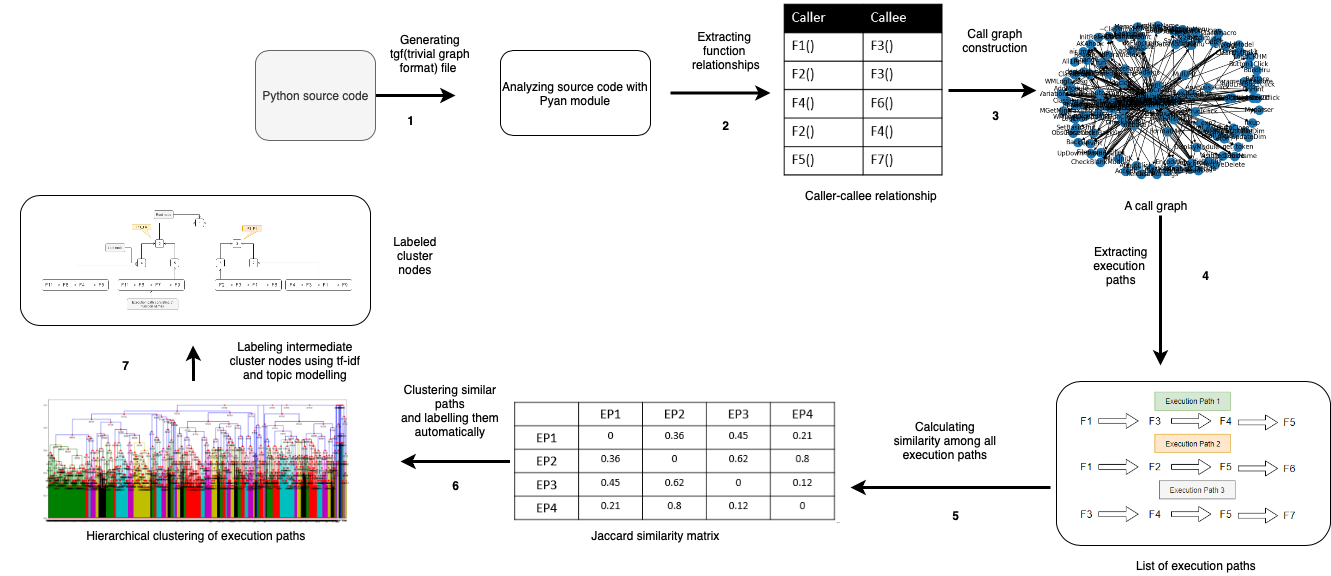
\includegraphics[width=\columnwidth]{figures/hla1/visual_tool_static_call_graph.png}
  \caption{Overview of the overall approach}~\label{hla1:fig:overall}
\end{figure*}

\subsubsection{Analyzing source code using modified Pyan module}

For extracting function relationships from a python system, we used a modified version of Python module Pyan \cite{pyan}. Pyan works only for a single directory. We adapted Pyan so that it can consider multiple directories while extracting the relationships. Pyan uses the abstract syntax tree (AST) for extracting function relationships. After analyzing the source code, we generated a graph in TGF (Trivial Graph Format). In TGF, all modules and functions' physical addresses in the source code are printed first. Then, relationships between all functions are presented as the caller and callee pair.

\subsubsection{Extracting function relationships from TGF}

Function relationships from the TGF file are used as inputs in our technique. Encoded unique identifiers are used to replace function names for ease of processing during the hierarchical clustering step.

\subsubsection{Static call graph creation based on the extracted relationships}
To perform different graph operations, we have created graph objects of the NetworkX \cite{networkx} module using the extracted function relationships. 
\subsubsection{Extracting execution paths}

The execution path is a simple path between an entry node and an exit node. An entry node is a node in the call graph which incoming edge degree is zero. Hence, no function is dependant on an entry node. An exit node is a node that has a zero degree of outgoing function calls. We have generated a list of entry and exit nodes to generate execution paths from a call graph. A simple path means no repeated node visit while visiting from the source node to the destination node. We have collected all possible simple paths for all possible combinations of entry node and exit node pairs. We have implemented a simple path finding algorithm from the NetworkX library, which uses a modified DFS algorithm for finding simple paths between a pair of nodes \cite{networkx}. For our task, a source node is an entry node, and a destination node is an exit node.    

\subsubsection{Distance matrix for execution paths}

For clustering execution paths (sequence of function names), we need to measure the similarity between all pairs of execution paths. For this purpose, we implemented the Jaccard similarity measure \cite{niwattanakul2013jaccardKeywordsSimilarity}. The linkage algorithm uses this similarity in the next step. If we have two sets $ A $ and $ B $, then their Jaccard similarity will be the ratio of their intersection's cardinality by the union. The clustering algorithms work on the distance, which is, in our case, the dissimilarity between two execution paths/clusters. We have subtracted the similarity score with one to get the dissimilarity value according to equation \ref{eq:jaccard}. After calculating dissimilarity between all pairs of execution paths, we converted the 2d matrix to 1d condensed matrix to make our program memory efficient.

\begin{equation}
Dis(A, B) = 1 - \frac{A\cap B}{A\cup B}
\label{eq:jaccard}
\end{equation}

\subsubsection{Clustering execution paths using linkage algorithms}

To group similar execution paths as clusters, we have implemented a linkage algorithm using popular python package Scipy \cite{scipy}. Scipy has different types of linkage algorithms already implemented in its core. To update the distance between two clusters, we have picked Ward the minimum variance method \cite{ward}. Equation \ref{eq:ward} shows how distance using the Ward method is updated when two clusters from cluster forest are merged into a new one \cite{scipy}.

\begin{equation}
     d(u, z) =   \sqrt{\frac{(n_x+n_z)d(x,z)^2+ (n_y+n_z)d(y,z)^2 - n_z d(x,y)^2 }{n_x+n_y+n_z}}
    \label{eq:ward}
\end{equation}

 
In equation \ref{eq:ward}, $u$ is a newly formed cluster, and $z$ is an unused cluster which will be used as reference to calculate distance. $n_x$, $n_y$ and $n_z$ are respectively the number of execution paths (as we are clustering the execution paths) in cluster $x$, $y$ and $z$.
When a new cluster $u$ is created, the distance between $u$ and all the other clusters are updated in the distance matrix. Additionally, cluster $x$ and $y$ are removed from the distance matrix as they have been merged as a new cluster $u$. This step is followed iteratively until only a single cluster remains in the cluster forest. 

For example, in Figure \ref{fig:motivation}, initially, at the start of the clustering process, there are four clusters 4, 5, 6, 7. Next, the hierarchical clustering algorithm selects the two most similar clusters (4, 5 ) to merge them as a new cluster 2. Now, in the clustering process, we have three clusters 2, 6, 7. Similar to the previous step, the most two similar clusters are merged into one. This process continues until there is only one cluster left. Ward method is used to calculate distance between the newly merged cluster with others.

% \vspace{4mm}
\subsection{Naming Nodes in an Abstract Code Summary Tree}
\label{hla1:node_title}
After getting a cluster tree from the previous step, our next step is to name the clusters to represent the high-level functionality of source code in a readable way. In this step, we will be able to locate high-level concepts in the ACS tree. However, each cluster has a list of function call sequences, and the function call sequences are called execution paths. Our challenge is to extract essential keywords from this collection so that developers can get an overview of the underlying high-level functionalities under the cluster. Naming the source artifacts correctly, in our case, which is nodes in the abstract code summary tree, is the fundamental contribution of this work. Proper naming can help developers to comprehend a program promptly. Toward the naming, we have applied three popular techniques used widely in natural language summarization tasks. These methods try to find meaningful and significant topics from a set of documents. In our approach, a document is an execution path that contains a list of function names. All the execution paths under a cluster are considered as documents.
A previous study used function names as terms in a document \cite{gharibi2018automaticStaticCluster}. However, we want to see what happens if we parse the function names and use the words in function names and use them as a term in documents. We used both words in a function name, and method names approach for the three techniques. In Section \ref{background:techniques}, we have discussed TFIDF, LDA and LSI techniques to generate node label.
% Below we briefly described how these three techniques work. 

% \subsubsection{TFIDF}
% TFIDF \cite{ramos2003usingTfidfRelevance} is a very popular information retrieval technique widely used in text-based search engines. The full form of the TFIDF is term frequency-inverse document frequency. Term frequency means how frequent a term in a document is. Term frequency is calculated according to equation \ref{eq:tf}.

% \begin{equation}
%     tf(t,d) = f_{t,d}
%     \label{eq:tf}
% \end{equation}
% \begin{equation}
%     idf(t) = \log(\frac{n}{df(t)})+1
%     \label{eq:idf}
% \end{equation}
% \begin{equation}
%     tf-idf(t,d) = tf(t,d) * idf(t)
%     \label{eq:TFIDF}
% \end{equation}
% The function $f_{t,d}$ counts frequency of term $t$ in the document $d$. Inverse document frequency is calculated according to equation \ref{eq:idf}. Function $df(t)$ in equation \ref{eq:idf} is the count of documents term $t$ is present. The main purpose of $idf$ is to penalize common keywords in the corpus. Term frequency (tf) and Inverse document frequencies (idf) are multiplied to get score for terms. We have adopted \texttt{TFIDFVectorizer} class of scikit-learn \cite{scikit-learn} library for implementing $TFIDF$ technique.
% \subsubsection{LDA}
% Latent Dirichlet Allocation (LDA) \cite{blei2003latentLDA} is a statistical model that tries to describe a set of documents by assuming they are created from some topics. LDA is a very popular topic modeling technique. LDA assumes every term in a document belongs to some topic. So, it assumes each term belongs to some topic and then performs analysis to find which assumptions are supported by statistics of the corpus. We have used Gensim \cite{gensim} library for implementing LDA for our approach.
% \subsubsection{LSI}
% Latent Semantic Indexing (LSI) \cite{deerwester1990indexingLSI} is a technique used in natural language processing. LSI assumes semantically similar words occur together. First, the term-document frequency matrix is calculated from the corpus. Then, this term-document frequency matrix is decomposed into three matrices using the Single Value Decomposition (SVD) technique. Terms are first assigned to topics using the term-document frequency matrix. Then, using all the topics, a topic importance matrix is derived, which leads to topics for the documents. Similar to LDA, we used Gensim \cite{gensim} library for implementing LSI. 

\begin{figure*}[h!]
    \begin{center}
    \subcaptionbox{Full abstract code summary tree with local view\label{fig:tool_ui}}
    {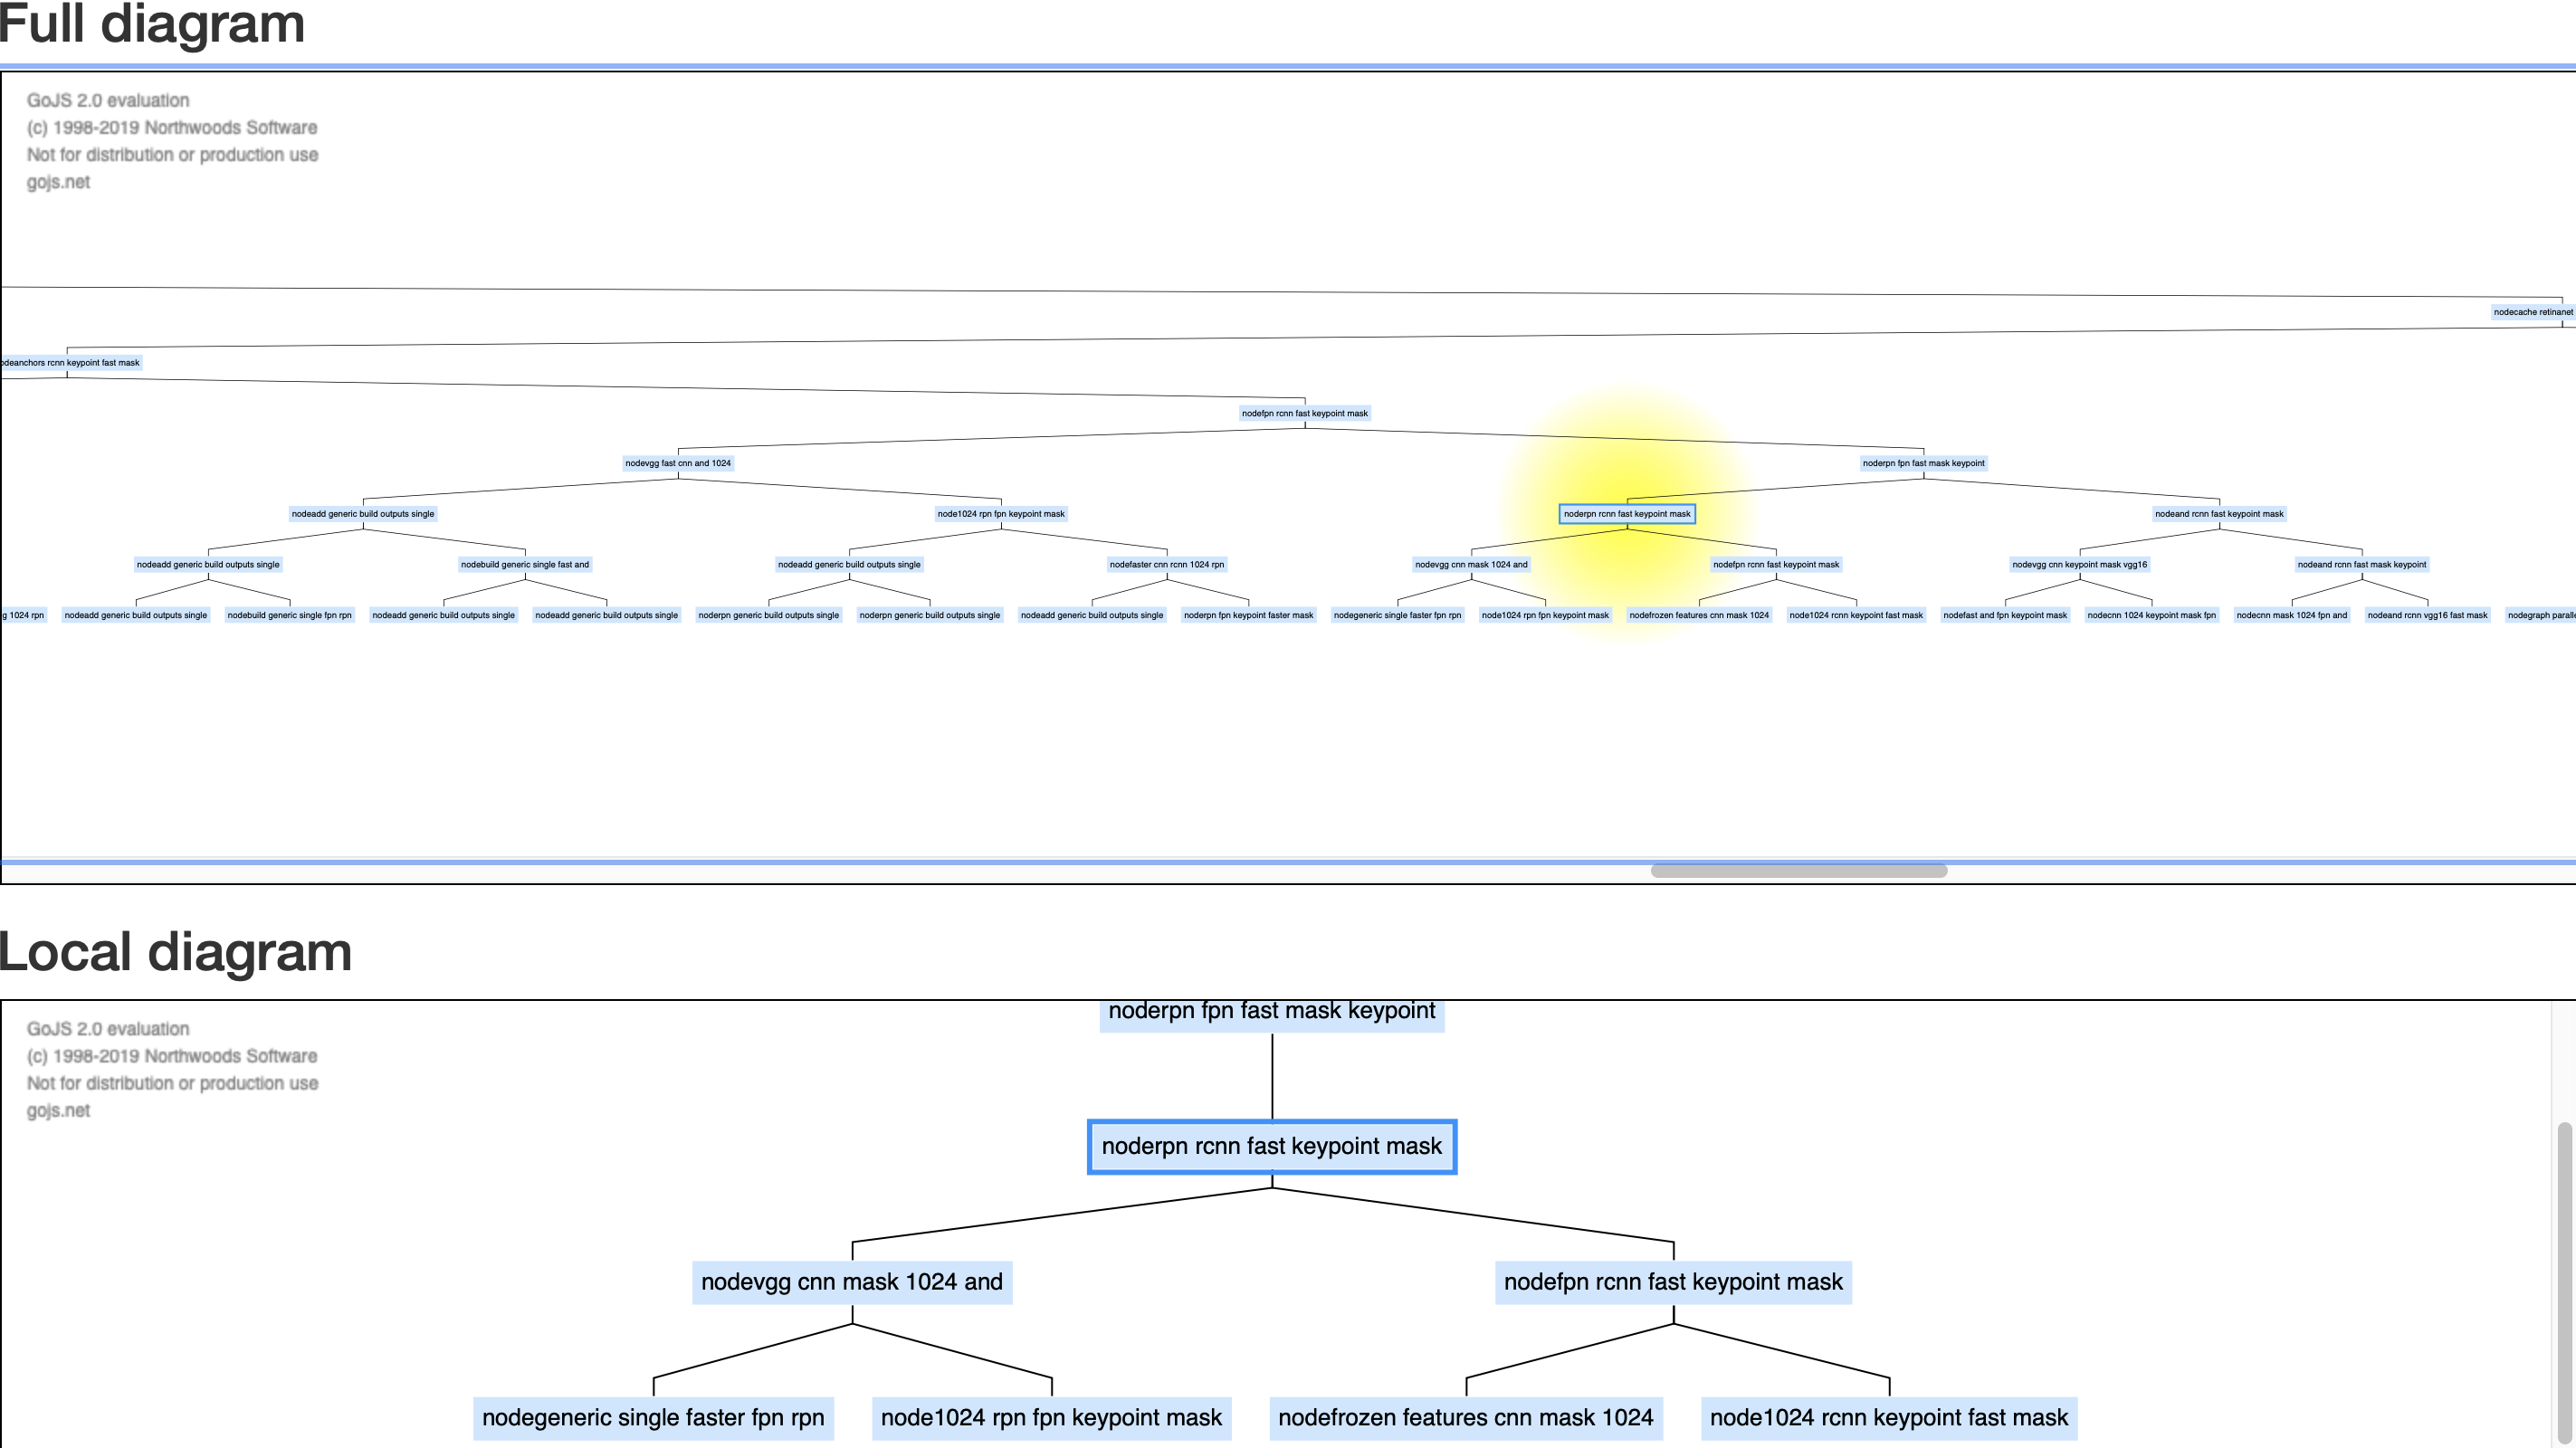
\includegraphics[scale=0.25]{figures/hla1/ToolUI.png}}
    \subcaptionbox{Form presented to the participants for answering\label{fig:userstudy}}
    {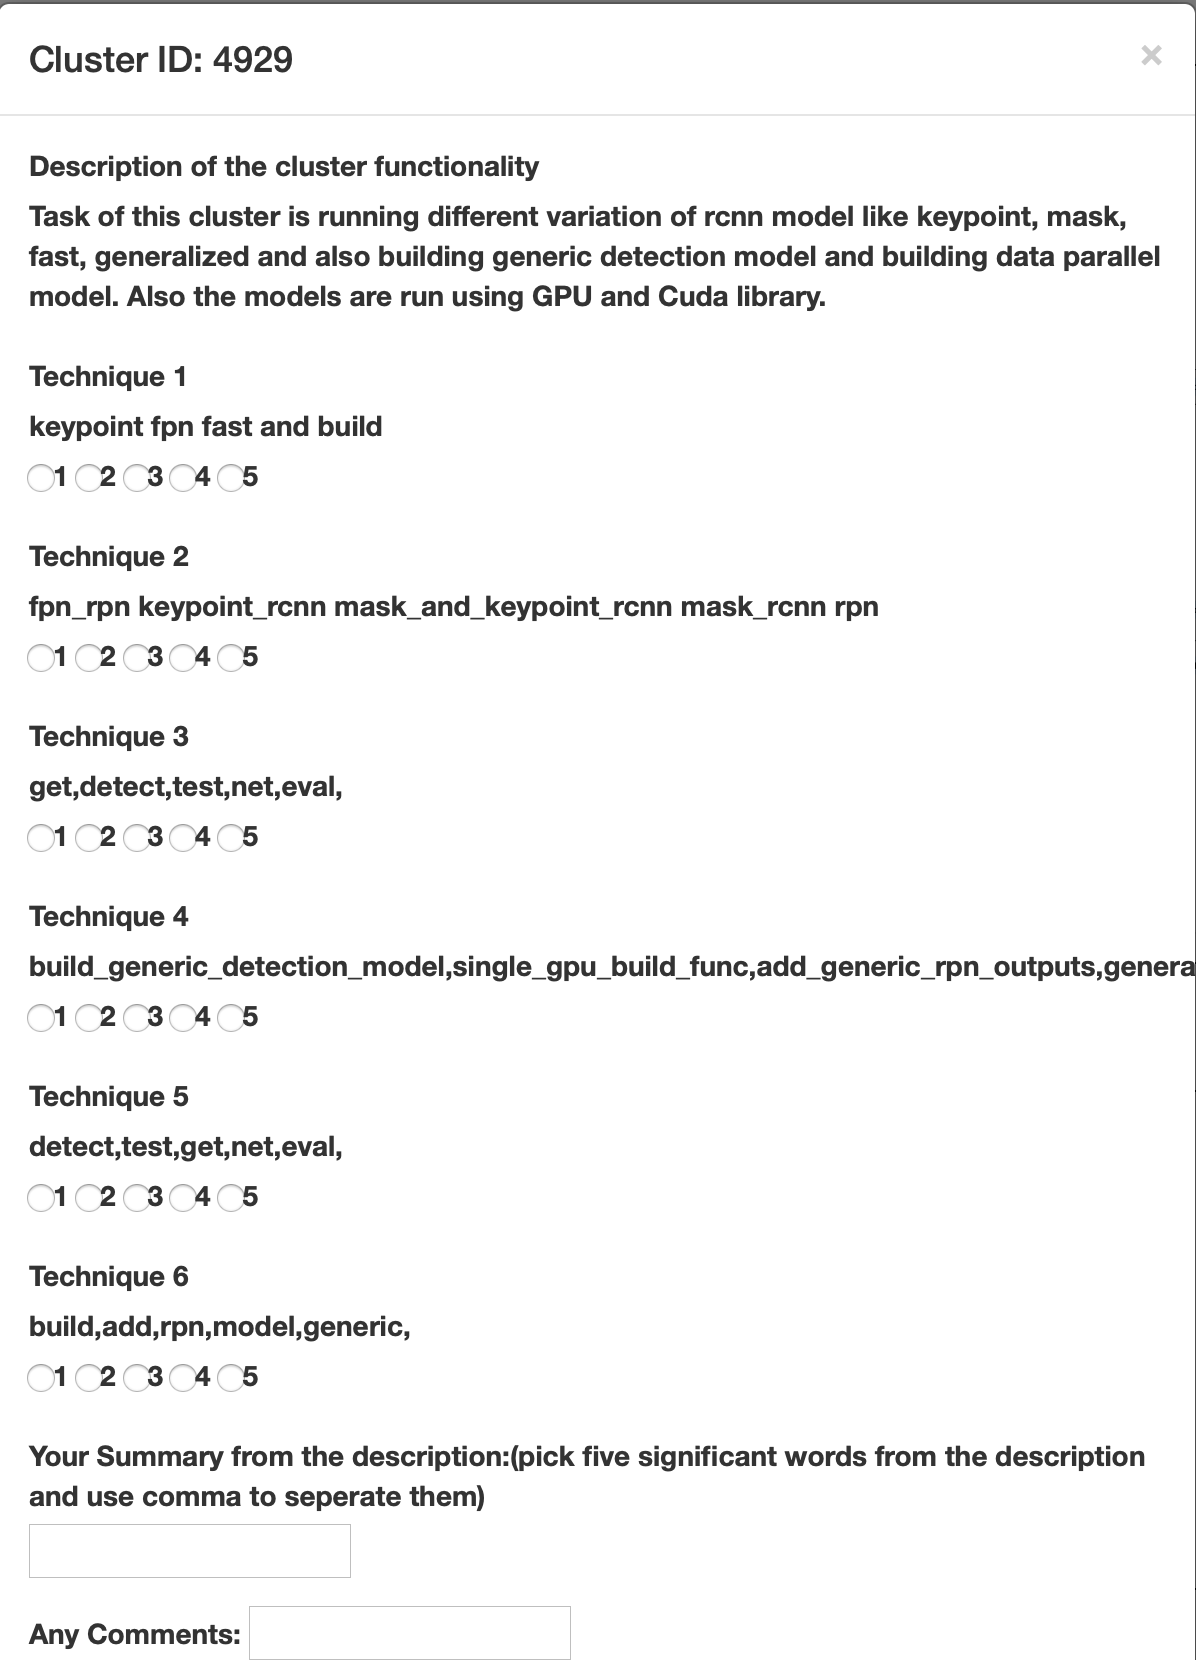
\includegraphics[scale=0.23]{figures/hla1/userstudy.png}}
    \caption{Tool UI presented to the study participants}
    \label{fig:tool}
    \end{center}
    
\end{figure*}

\section{Experimental Design}
\label{Experimental}
This section will discuss the research questions that need to be answered regarding the abstract code summary tree, how we collected our subject systems for the experiment, and details about users who participated in this study.

\subsection{Research questions}
We want to explore how manual naming supports automatic naming techniques. To investigate this, we set \texttt{RQ1}.
Besides, we have compared developer preferences for three different techniques using function names as terms by \texttt{RQ2}. Similarly, for \texttt{RQ3}, we changed the input for information retrieval techniques by words in function names instead of function names and compared developers' ratings among the three approaches. Finally, we want to see the performances of our two variations of choosing terms by a systematic comparison by \texttt{RQ4}. 

\begin{itemize}
    \item \textbf{\texttt{RQ1}} How well does the automatic labeling perform using the candidate approaches compared to manual labeling?  (To evaluate this, we will use pyramid measure)
    \item \textbf{\texttt{RQ2}} How do developers evaluate different labeling approaches based on function names?
    \item \textbf{\texttt{RQ3}} How do developers evaluate different labeling approaches based on words in method names? 
    \item \textbf{\texttt{RQ4}} How can we compare the preferences of developers between the two approaches addressed in \texttt{RQ2} and \texttt{RQ3}? 
\end{itemize}


\subsection{Dataset Collection}
In order to conduct the user-study, we have collected source code of three popular Python projects \texttt{Detectron}~\cite{Detectron2018}, \texttt{Real\-Time\-Voice\-Cloning} \cite{realTime} and \texttt{requests}~\cite{requests}. The reason behind choosing these subject systems for our study is that they are popular among Python developer communities. These projects follow the standard conventions of software developments so participants will be able to relate keywords from their day-to-day knowledge. Additionally, open-source projects tend to follow proper function naming conventions, which is important for our approach as it completely depends on function names. We extracted source code and applied the steps described in Section \ref{alg:overall}. We have printed clusters with their corresponding execution paths and names suggested by the candidate techniques in a file for doing the user-study. We have chosen 12 clusters semi-randomly, i.e.,  four from each of the subject systems, which ensures the coverage of different levels' clusters. 


\subsection{User-study}
For the 12 clusters, we manually analyzed each cluster's execution paths and come up with a 2-3 line description of what happens inside the clusters. Before the study, we told users to rate the automatic summaries of our three techniques, each with two variations. Additionally, we also provided a text box for the participants to select five keywords from the description produced by manual analysis of execution paths. We have used this summary to compute the Pyramid score for the three techniques of the words in function name variation. A total of five persons participated in the study with a software development background. Among them, three are female, and two are male. Each of the participants has at least a Bachelor's degree in Computer Science. Two of them are graduate students, and the other three are working as developers in three different software firms. All of them have at least three years of experience in programming experience with an average of 3.8 year. 


In Figure \ref{fig:tool_ui}, the abstract code summary tree from our tool is presented. The upper box contains the full abstract code summary tree. Below the concept tree, a local view can be used to look closer to the concept cluster. Developers can click on any node in the concept diagram to get a zoomed view of its child and parents. 

In Figure \ref{fig:userstudy}, a screenshot of the form provided to the participants is presented. When participants right-click on the target clusters, a form with cluster id and a brief description of the execution paths' manual analysis is popped up. In the form, we asked the participants about their preference (1 means least preferred, 5 means most preferred) for names suggested by the six techniques and selected five keywords from the descriptions to complete the study.

\begin{table*}[h]
\small
\caption{Pyramid score computation }
\label{table-pyramid1}
\centering
\begin{tabular}{|l|l|l|l|l|l|l|l|l|l|l|l|l|}
\hline
  & response & request &	dict &	send &	from &	build &	cookiejar &	create &	get &	cookie &	prepare &	merge  \\ \hline
D1 & x      & x     & x           & x   & x    &        &         &     &      &    &  &    \\ \hline
D2 &     x   &      &  x       &     &    & x      & x       &   &      & x& &       \\ \hline
D3 & x      &       &           &    &     &    x    &         & x   &  x    & x & &     \\ \hline
D4 &        &       &             &   x  &     &        &        &     & x    & x    & x &    \\ \hline
D5 &  x     &      &    x         &     &     &        &        & x    &     & x    &  &   \\ \hline
\texttt{TFIDF\_word}  &   x(4)     &       &             &  x(2)   &  &        &     &     &  &  & & x(1)    \\ \hline
\texttt{LDA\_word}  &        &   x(1)    &             &     &  &        &     &     & x(2) &   & x(1) &  \\ \hline
\texttt{LSI\_word}  &        &   x(1)    &             &  x(2)   &   &        &  x(1)     &     & x(2) &  & & \\ \hline
\end{tabular}
\end{table*}

\section{Results and Discussion}
\label{results}
% \vspace{3mm}

\begin{figure*}[h]
 \pgfplotstableread{
 1 0.7857 0.71 0.29
2 0.71 0.29 0.14
3 0.53 0.06 0.06
4 0.56 0.125 0.125
5 0.61 0.46 0.15
6 0.57 0.05 0.315
7 0.9 0.72 0.09
8 0.53 0.53 0.46
9 0.43 0.31 0
10 0.46 0.26 0.4
11 0.81 0.5 0.43
12 0.73 0.4 0.33
}\dataset
% \resizebox{6.0in}{!}{
\begin{tikzpicture} \begin{axis}[xbar,
ylabel={\#Cluster no.},
xlabel={Pyramid score},
 symbolic y coords={1, 2, 3, 4, 5, 6, 7, 8, 9, 10, 11, 12},
        ytick=data,
        nodes near coords, 
        nodes near coords align={horizontal},
        bar width=0.18cm,
width=\textwidth,
% height=7.5cm,
xmin=0,
xmax=1.0, 
xticklabel style={font=\footnotesize},
yticklabel style={font=\footnotesize, /pgf/number format/fixed},
y tick label style={ rotate=0},
major y tick style = {opacity=0},
minor y tick num = 1,
minor tick length=1ex,
xmajorgrids = true,
%grid=both,
%grid style={line width=.1pt, draw=black!10},	
legend entries={TFIDF\_word,LDA\_word, LSI\_word},	
legend style={at={(0.5,-0.1)},
anchor=north,
legend columns=6,
font=\scriptsize,
% text width=2.75in,
% minimum height=0.20in,
nodes near coords
}
        ]
    \addplot [draw=black!100, fill=black!10] table[x index=1,y index=0] \dataset;
    \addplot [draw=black!100, fill=black!30] table[x index=2,y index=0] \dataset;
    \addplot [draw=black!100, fill=black!50] table[x index=3,y index=0] \dataset;
    
\end{axis}
\end{tikzpicture}
% }
  \caption{Pyramid score of the 12 clusters}~\label{fig:pyramid12}
\end{figure*}


\subsection{User Naming vs. Automatic Naming}

To investigate how automatic naming accords with manual naming, we have used Pyramid score \cite{nenkova2004evaluating}. Pyramid score is used in natural text summarization tasks to compare an automatic summary with a manual summary. Haiduc et al. \cite{haiduc2010supporting}  used Pyramid score to support source code summary with developers' summary, which motivated us to adopt Pyramid score to find out how our automatic approaches of abstraction harmonize with developers' selections. In Table \ref{table-pyramid1}, we have shown the Pyramid score calculation process for a cluster (i.e., cluster number 10 of the 12 clusters). The preferences of five developers who participated in this study are represented by D1,\ldots, D5. X\_word represents the corresponding outputs of $X \in {TFIDF, LDA, LSI }$ by considering words in function names. Each column presents unique keywords from the selections of five participants. Furthermore, we have marked which words are matched with the automatic summary from a developers' summary in the corresponding cells. In each row for the automatic techniques, we have put the support from five developers for keywords being present in the summary.



For example, we can see that keyword $response$ is present in TFIDF with words in the function name variation, and four of the developers picked $response$ in their summary. So, support for keyword $response$ is given 4. To get the Pyramid score for cluster number 10, we have summed each keyword's support in automatic naming by developers. In this case, values are $4(response), 2(send), 1(merge)$. We divide the sum of these support values by the top five most frequent keywords of five developers' summary. So, the score is now $(4+2+1)/(4+4+3+2+2) = 0.466 $ for cluster 10. Greater Pyramid score means that the automatic naming is becoming more human in our case. In Figure \ref{fig:pyramid12}, we have plotted Pyramid score for 12 clusters with the three techniques of word variant and support of the five participants for them. In the figure, we can see that for most of the clusters, the \texttt{TFIDF\_word} based automatic naming technique's summary agrees more compared to other techniques with  the developers' provided summaries.



% \vspace{3mm}
\subsection{User Rating on Function Name Variant}
To answer the RQ2, we use the techniques with function names as unit variation. We asked our participants to rank each technique's summary with a score ranging from 1 to 5 to reflect how well they support the manual description. In Figure \ref{fig:method}, we have plotted the average ranking of the participants for 12 clusters with the techniques. In the figure, we can see the users preferred LSI naming technique over the LDA. LSI is preferred in almost 50\% of the clusters. For clusters 1, 4, 9, participants' preference for LDA and LSI are the same. The reason is that both techniques provided a similar kind of summary for the cluster in the automatic naming process.

\begin{figure*}[h]
\pgfplotstableread{
 1	2.6	3	3
 2	3.4	2.8	4
 3	2.8	2.8	3.4
 4	3	3.2	3.2
 5	3.2	3	2.6
 6	3.2	2.2	2.8
 7	3.2	2.8	3.2
 8	3.4	2.8	3.2
 9	3.2	3.4	3.4
 10	3	3.4	3.6
 11	3	3.8	3.2
 12	3.6	3.4	3
}\dataset
\resizebox{6.0in}{!}{
\begin{tikzpicture}
\begin{axis}
[ybar,
% enlargelimits=0.05,
bar width=0.10cm,
width=0.55\textwidth,
height=4.5cm,
ymin=0,
ymax=5.0, 
ylabel={Average ranking of
five participants},
xlabel = {\#Cluster no.},
yticklabel style={font=\footnotesize},
xticklabel style={font=\footnotesize, /pgf/number format/fixed},
xtick=data,
xticklabels = {1, 2, 3, 4, 5, 6, 7, 8, 9, 10, 11, 12},
x tick label style={ rotate=45},
major x tick style = {opacity=0},
minor x tick num = 1,
minor tick length=1ex,
ymajorgrids = true,
label style={font=\footnotesize},
%grid=both,
%grid style={line width=.1pt, draw=black!10},	
legend entries={TFIDF(function names),LDA(function names), LSI(function names)
},	
legend style={
at={(0.5,-0.35)},
anchor=north,
legend columns=-1,
font=\scriptsize,
%text width=2.75in, 
minimum height=0.20in,
nodes near coords style={rotate=90,  anchor=west, font=\tiny},
nodes near coords
},
]
% \addplot[draw=black!100, fill=green!20,pattern= grid] table[x index=0,y index=1] \dataset;
\addplot[draw=black!100, fill=black!10] table[x index=0,y index=1] \dataset;
\addplot[draw=black!100, fill=black!30] table[x index=0,y index=2] \dataset;
\addplot[draw=black!100, fill=black!50] table[x index=0,y index=3] \dataset;
\end{axis}
\end{tikzpicture}
}
\caption{User preference among three implemented naming techniques (considering methods as terms)}
\label{fig:method}
% \vspace{-2mm}
\end{figure*}

\begin{figure*}[h!]
\pgfplotstableread{
1	3.4	3.4	3
 2	3.4	3.2	3
 3	3	3.2	2.8
 4	3.2	3	3.2
 5	3.4	3.8	3
 6	3.6	3.4	3.8
 7	3.6	3.6	3.6
 8	3.2	3	3.6
 9	4	3.4	4.2
 10	3.6	3.6	4
 11	3.8	3.6	3.8
 12	3.8	3.8	3.4
}\dataset
\resizebox{6.0in}{!}{
\begin{tikzpicture}
\begin{axis}
[ybar,
% enlargelimits=0.05,
bar width=0.10cm,
width=0.55\textwidth,
height=4.5cm,
ymin=0,
ymax=5.0, 
ylabel={Average ranking of
five participants},
xlabel = {\#Cluster no.},
yticklabel style={font=\footnotesize},
xticklabel style={font=\footnotesize, /pgf/number format/fixed},
xtick=data,
xticklabels = {1, 2, 3, 4, 5, 6, 7, 8, 9, 10, 11, 12},
x tick label style={ rotate=45},
major x tick style = {opacity=0},
minor x tick num = 1,
minor tick length=1ex,
ymajorgrids = true,
label style={font=\footnotesize},
%grid=both,
%grid style={line width=.1pt, draw=black!10},	
legend entries={TFIDF(words in function names),LDA(words in function names), LSI(words in function names)
},	
legend style={
at={(0.5,-0.35)},
anchor=north,
legend columns=-1,
font=\scriptsize,
% text width=2.75in,
minimum height=0.20in,
nodes near coords style={rotate=90,  anchor=west, font=\tiny},
nodes near coords
},
]
\addplot[draw=black!100, fill=black!10] table[x index=0,y index=1] \dataset;
\addplot[draw=black!100, fill=black!30] table[x index=0,y index=2] \dataset;
\addplot[draw=black!100, fill=black!50] table[x index=0,y index=3] \dataset;
\end{axis}
\end{tikzpicture}
}
\caption{User preference among three implemented naming techniques (considering words in methods as terms)}
\label{fig:word}

\end{figure*}

\begin{figure*}[h!]
  \pgfplotstableread{
  

  1 3.5 3.133333333
  2 3.416666667 3.05
  3 3.45 3.216666667
}\dataset
\begin{tikzpicture}
\begin{axis}[xbar,
bar width=0.50cm,
% ylabel={\#Cluster no.},
% xlabel={Pyramid score},
yticklabel style={font=\footnotesize},
xticklabel style={font=\footnotesize, /pgf/number format/fixed},
xmin = 0,
xmax = 5.0,
yticklabels = {TFIDF, LDA, LSI},
%  symbolic y coords={TFIDF, LDA, LSI},
        ytick=data,
        legend entries={words\_in\_function\_names, function\_names},	
         nodes near coords, 
        nodes near coords align={horizontal},
legend style={
at={(0.5,-0.15)},
anchor=north,
legend columns=-1,
font=\scriptsize,
%text width=2.75in,
minimum height=0.20in}
]
    \addplot [draw=blue,
        pattern=horizontal lines ,
    ] table[x index=1,y index=0] \dataset;
    \addplot [draw=green,
        pattern=crosshatch ,
    ] table[x index=2,y index=0] \dataset;
\end{axis}
\end{tikzpicture}
  \caption{Comparison between three techniques considering function names and words in function names}~\label{fig:method_vs_word}
\end{figure*}

\subsection{User Rating on Words in Function Name Variant}
We have followed a similar approach to answer RQ3 that we used to answer RQ2. We averaged five participants' rankings for 12 clusters for the three techniques (TFIDF, LDA, LSI). In RQ3, we want to know participants' preference when we consider words in the function names as unit for the TFIDF, LDA, LSI-based techniques. In Figure \ref{fig:word}, we have plotted user rankings of the automatically suggested names for 12 clusters. Among twelve clusters, we can see that in seven of them, developers preferred names suggested by TFIDF and LSI technique in preference to the LDA technique, which covers almost 60\% of the clusters. Therefore, \texttt{RQ3} can be answered to establish that words in function name variation perform better with TFIDF, LSI than LDA.      



\subsection{Function Name vs. Words in Function Name}
For \texttt{RQ4}, we want to see users' preference on TFIDF, LDA, and LSI based techniques of the two variations we mentioned in \texttt{RQ2} and \texttt{RQ3}.
So, we averaged the user rankings of 12 clusters of three techniques from Figure \ref{fig:method} and Figure \ref{fig:word}. In Figure \ref{fig:method_vs_word}, we plotted the average ranks of the three techniques in two variations (i.e.,function\_names and  words\_in\_function\_names). From the figure, we can observe that developers preferred TFIDF, LDA, and LSI techniques with word as unit over method name variations. Words in function names variation get at least 5\% higher preference than the method names variations for each of the three techniques. 

% \section{Related Work}
% \label{relatedwork}
% Feng \textit{et al.} \cite{feng2018hierarchicalExecutionComprehension} proposed an approach to abstract execution traces for program comprehension. To get execution traces, they used BLINKY to instrument source code for getting method-invocation calls. Different test cases are used to generate execution traces for different scenarios. From dynamic logs, they have built phase trees that are created from caller-callee relationships of invoked methods. After deleting duplicate phases, they clustered unique phases using the Agglomerative hierarchical clustering algorithm. Next, they applied a mining technique to get frequent pattern phases of each level of clustered phase tree. For comprehension purposes, they used TFIDF to rank method names of frequent phases and then used the top 20 method names for the final label. Depending on dynamic call graphs comes with some limitations as it depends on the test cases heavily, and the size of log file generated is difficult to handle. Therefore, we choose static call graphs to remove the test dependency and capture a call graph's overall execution scenario. Gharib \textit{et al.}  \cite{gharibi2018automaticStaticCluster} proposed an approach using static call graphs for hierarchical abstraction. First, they generated a static call graph for a subject system that captures overall function relationships. Second, execution paths from the call graph are extracted, which become the building blocks for their approach. Next, execution paths are clustered together to create abstract code summary of the target subject systems. Feng \textit{et al.}~\cite{feng2018hierarchicalExecutionComprehension} also named the clusters by extracting keywords from the function names present in execution paths. In their study, only the TFIDF technique is applied to extract and name intermediate clusters.

% For this study, our motivation is to take forward this approach and enrich it with existing techniques from the literature. Two limitations of the study from Gharib \textit{et al.}  are using only TFIDF method for information retrieval and no presence of user study to validate how developers prefer the output abstractions. We adopt two more topic modeling techniques for information retrieval, which show promising results for naming source code artifacts in the literature \cite{de2012IRMethodsArtifacts}. Andrea \textit{et al.}  \cite{de2012IRMethodsArtifacts} tried to apply IR techniques like VSM, LDA, and LSI on  source code artifacts. To evaluate IR techniques' effectiveness, they also produced suggestions from 17 users on the same classes. Then, they assessed the performance of automatic naming by comparing overlap
% with manual naming of users. In their study, authors also find that heuristic based approaches focusing on function signatures perform well for code artifacts summarization. Inspired from their study, we use LDA and LSI on function signatures to extract concepts in code in this study. Another improvement from Gharib \textit{et al.} is to adopt a user study for validating automatic abstraction. Sonia \textit{et al.}  \cite{haiduc2010supporting} used Pyramid score to evaluate the output of automatic code summary with developers' summary. We also adopt this Pyramid score, which is widely used for the evaluation of natural language summaries. 

\section{Threats to Validity}
We have used three subject systems for the user study, and all of them are written with the Python language. We acknowledge that our user sample size is small. To mitigate the effect of randomness, we used three different systems, considered four clusters from each of them and invited experienced developers for the study. Our approach depends on function names. Therefore, our approach would be less successful when the naming conventions are not properly followed. We have used open-source projects which generally maintain good naming conventions.  We have collected user summary after they evaluated six techniques to understand the limitation of automatic naming and provide feedback accordingly.  
% \vspace{6mm}
\section{Summary and Discussion}
\label{conclusion}
While proposing an approach to find concepts in source code from static call graph analysis, we try to remove the shortcomings of existing approaches in terms of techniques evaluation and use cases. We use two different variations of terms to recommend concepts that leverage developers' program perception effort while understanding a system. As program comprehension is a subjective matter, we collect user data to evaluate how our automatic labeling approach accords with user choice. The techniques we use are TFIDF, LDA, and LSI, with two variations (i. e., naming by function names, and naming by words in function names), where we found the TFIDF works better in cluster naming, and users prefer words in functions variants.   

During our manual analysis to generate a brief description of twelve clusters by observing execution paths, we found patterns in execution paths that might make the naming of concept cluster more human. In the next chapter, we will explore how we can generate more information for abstraction nodes.
